\documentclass{article}



\usepackage{fullpage}
\usepackage{nopageno}
\usepackage{amsmath}
\usepackage{amsfonts}
\usepackage{graphicx}
\usepackage{framed}
\usepackage{xcolor}

\definecolor{dark_red}{rgb}{0.5,0.0,0.0}
\definecolor{dark_green}{rgb}{0.0,0.5,0.0}
\definecolor{dark_blue}{rgb}{0.0,0.0,0.5}

\newcommand{\dr}[1]{\textcolor{dark_red}{#1}}
\newcommand{\dg}[1]{\textcolor{dark_green}{#1}}
\newcommand{\db}[1]{\textcolor{dark_blue}{#1}}


\begin{document}

\section*{Solving Simultaneous Equations}

Given two variables \(x\) and \(y\) whose values are sought, the values of \(x\) and \(y\) are often, but not always, uniquely determined by 2 simultaneous equations, referred to as a system of equations:
\[\left\{\begin{array}{c} f_1(x,y) = g_1(x,y) \\ f_2(x,y) = g_2(x,y) \end{array}\right.\]
where \(f_1(x,y)\), \(g_1(x,y)\), \(f_2(x,y)\), and \(g_2(x,y)\) are arbitrary expressions.



\subsection*{Case: Independent equations}

It is a relatively simple matter to find \(x\) and \(y\) when the equations are independent, which is to say that each equation contains 1 variable:
\[\left\{\begin{array}{c} f_1(x) = g_1(x) \\ f_2(y) = g_2(y) \end{array}\right.\]
The equations \(f_1(x) = g_1(x)\) and \(f_2(y) = g_2(y)\) can be solved separately to find the values of \(x\) and \(y\) respectively. As an example, consider the system:
\[\left\{\begin{array}{c}
5x + 4 = 2x - 20 \\
-4y + 10 = 3y - 4
\end{array}\right.\]
The top and bottom equations can be independently solved:
\[5x + 4 = 2x - 20 \iff 3x + 4 = -20 \iff 3x = -24 \iff x = -8\]
\[-4y + 10 = 3y - 4 \iff -7y + 10 = -4 \iff -7y = -14 \iff y = 2\]
to get \(x = -8\) and \(y = 2\).



\subsection*{Case: One of the equations has only 1 variable}

Moving to more complicated scenarios, now one equation will contain one variable, while the other equation contains both variables. When, for example, the first equation contains only \(x\), the general form is:
\[\left\{\begin{array}{c} f_1(x) = g_1(x) \\ f_2(x,y) = g_2(x,y) \end{array}\right.\]
The first equation \(f_1(x) = g_1(x)\) is solved to find \(x\). With the value(s) of \(x\) known, substituting the value of \(x\) into the second equation \(f_2(x,y) = g_2(x,y)\) yields an equation that contains only variable \(y\). This equation can now be solved for the value(s) of \(y\). As an example, consider the system:
\[\left\{\begin{array}{c}
-x + 6 = 9 \\
x + 5y = 7
\end{array}\right.\]
The top equation contains only variable \(x\), and can be solved for \(x\):
\[-x + 6 = 9 \iff -x = 3 \iff x = -3\]
with the knowledge that \(x = -3\), the bottom equation becomes an equation that contains only \(y\), and can be solved for \(y\):
\[x + 5y = 7 \iff -3 + 5y = 7 \iff 5y = 10 \iff y = 2\]



\subsection*{Case: Both equations have 2 variables}

The most complicated scenario occurs when variables \(x\) and \(y\) appear in both equations:
\[\left\{\begin{array}{c} f_1(x,y) = g_1(x,y) \\ f_2(x,y) = g_2(x,y) \end{array}\right.\]
In this scenario, one of the equations can be solved to express one variable as an expression involving the other variable. For example, the equation \(f_1(x,y) = g_1(x,y)\) can be manipulated to express variable \(y\) as an expression of \(x\): \(y = h(x)\). With the knowledge that \(y = h(x)\), variable \(y\) can be replaced with \(h(x)\) in the second equation:
\[f_2(x,y) = g_2(x,y) \iff f_2(x,h(x)) = g_2(x,h(x))\]
The equation \(f_2(x,h(x)) = g_2(x,h(x))\) can be solved for \(x\). With the value(s) of \(x\) known, the corresponding values of \(y\) are computed by \(y = h(x)\).


\subsubsection*{Example 1}

Consider the system:
\[\left\{\begin{array}{c} 
3x + 4y = -2 \\
-x + 3y = 5
\end{array}\right.\] 
Choose any equation and any variable to solve for from this equation. For instance, choose the second equation and solve for \(y\) from this equation:
\[-x + 3y = 5 \iff 3y = x + 5 \iff y = (1/3)x + 5/3\]
It is now known that \(y = (1/3)x + 5/3\), and that this fact was derived from the second equation. Replacing \(y\) in the first equation gives:
\begin{align*}
& 3x + 4y = -2 
\iff 3x + 4((1/3)x + 5/3) = -2 
\iff 3x + ((4/3)x + 20/3) = -2 \\
\iff & (13/3)x = -26/3 \iff x = -2
\end{align*}
Knowing that \(x = -2\), 
\[y = (1/3)x + 5/3 = -2/3 + 5/3 = 1\]
Therefore:
\[(x, y) = (-2, 1)\] 
%\[x = -2 \;\wedge\; y = 1\]


\subsubsection*{Example 2}

Consider the system:
\[\left\{\begin{array}{c} 
2x + 3y = 1 \\
-7x - 11y = -1
\end{array}\right.\] 
Choose any equation and any variable to solve for from this equation. For instance, choose the first equation and solve for \(x\) from this equation:
\[2x + 3y = 1 \iff 2x = -3y + 1 \iff x = -(3/2)y + 1/2\]
It is now known that \(x = -(3/2)y + 1/2\), and that this fact was derived from the first equation. Replacing \(x\) in the second equation gives:
\begin{align*}
& -7x - 11y = -1 
\iff ((21/2)y - 7/2) - 11y = -1 
\iff -(1/2)y = 5/2 \\
\iff & y = -5
\end{align*}
Knowing that \(y = -5\), 
\[x = -(3/2)y + 1/2 = 15/2 + 1/2 = 8\]  
Therefore:
\[(x, y) = (8, -5)\]
%\[x = 8 \;\wedge\; y = -5\]


\subsubsection*{Example 3}

Consider the system:
\[\left\{\begin{array}{c} 
-9x + y = -1 \\
-16x + 2y = 2
\end{array}\right.\] 
Choose any equation and any variable to solve for from this equation. For instance, choose the first equation and solve for \(y\) from this equation:
\[-9x + y = -1 \iff y = 9x - 1\]
It is now known that \(y = 9x - 1\), and that this fact was derived from the first equation. Replacing \(y\) in the second equation gives:
\begin{align*}
& -16x + 2y = 2 
\iff -16x + (18x - 2) = 2 
\iff 2x = 4 
\iff x = 2
\end{align*}
Knowing that \(x = 2\), 
\[y = 9x - 1 = 17\]
Therefore:
\[(x, y) = (2, 17)\]
%\[x = 2 \;\wedge\; y = 17\]


\subsubsection*{Example 4}

Consider the system:
\[\left\{\begin{array}{c} 
3x - y = 5 \\
6x - 2y = 10
\end{array}\right.\] 
Choose any equation and any variable to solve for from this equation. For instance, choose the first equation and solve for \(y\) from this equation:
\[3x - y = 5 \iff -y = -3x + 5 \iff y = 3x - 5\]
It is now known that \(y = 3x - 5\), and that this fact was derived from the first equation. Replacing \(y\) in the second equation gives:
\begin{align*}
& 6x - 2y = 10 
\iff 6x + (-6x + 10) = 10 
\iff 0 = 0
\end{align*}
This equation is always true and places no constraint on the value of \(x\). \(x\) can therefore be any real number. Choosing a specific value of \(x\), the value of \(y\) must be \(y = 3x - 5\). Therefore the set of possible solutions is the set of all points that lie on the line:
\[y = 3x - 5\] 


\subsubsection*{Example 5}

Consider the system:
\[\left\{\begin{array}{c} 
x - 7y = 0 \\
-3x + 21y = 1
\end{array}\right.\] 
Choose any equation and any variable to solve for from this equation. For instance, choose the first equation and solve for \(y\) from this equation:
\[x - 7y = 0 \iff -7y = -x \iff y = (1/7)x\]
It is now known that \(y = (1/7)x\), and that this fact was derived from the first equation. Replacing \(y\) in the second equation gives:
\begin{align*}
& -3x + 21y = 1 
\iff -3x + 3x = 1 
\iff 0 = 1
\end{align*}
This equation is always false, and assuming the truth of the two equations has resulted in a contradiction. Therefore both equations cannot be simultaneously true, and there are {\bf no solutions}.


\subsubsection*{Example 6}

Consider the system:
\[\left\{\begin{array}{c} 
-2x + 3y = 2x - 2y - 35 \\
x + y = 49 - 7x + 8y
\end{array}\right.\] 
Choose any equation and any variable to solve for from this equation. For instance, choose the first equation and solve for \(y\) from this equation:
\[-2x + 3y = 2x - 2y - 35 \iff -2x + 5y = 2x - 35 \iff 5y = 4x - 35 \iff y = (4/5)x - 7\]
It is now known that \(y = (4/5)x - 7\), and that this fact was derived from the first equation. Replacing \(y\) in the second equation gives:
\begin{align*}
& x + y = 49 - 7x + 8y 
\iff x + ((4/5)x - 7) = 49 - 7x + ((32/5)x - 56) \\
\iff & (9/5)x - 7 = -(3/5)x - 7 
\iff (12/5)x = 0 
\iff x = 0
\end{align*}
Knowing that \(x = 0\), 
\[y = (4/5)x - 7 = -7\]
Therefore:
\[(x, y) = (0, -7)\]


\subsubsection*{Example 7}

Consider the system:
\[\left\{\begin{array}{c} 
2x + 2y + 2 = 3x + 3 \\
3x + 3y + 3 = 10y + 2
\end{array}\right.\] 
Choose any equation and any variable to solve for from this equation. For instance, choose the first equation and solve for \(y\) from this equation: 
\[2x + 2y + 2 = 3x + 3 \iff 2x + 2y = 3x + 1 \iff 2y = x + 1 \iff y = (1/2)x + 1/2\]
It is now known that \(y = (1/2)x + 1/2\), and that this fact was derived from the first equation. Replacing \(y\) in the second equation gives:
\begin{align*}
& 3x + 3y + 3 = 10y + 2 
\iff 3x + ((3/2)x + 3/2) + 3 = (5x + 5) + 2 
\iff (9/2)x + 9/2 = 5x + 7 \\
\iff & -(1/2)x = 5/2 
\iff x = -5
\end{align*}
Knowing that \(x = -5\), 
\[y = (1/2)x + 1/2 = -5/2 + 1/2 = -2\]
Therefore:
\[(x, y) = (-5, -2)\]


\subsubsection*{Example 8}

Consider the system:
\[\left\{\begin{array}{c} 
x - y + 3 = -2x + y - 4 \\
-2x + y - 5 = 3x - 2y + 10
\end{array}\right.\] 
Choose any equation and any variable to solve for from this equation. For instance, choose the first equation and solve for \(y\) from this equation: 
\begin{align*}
& x - y + 3 = -2x + y - 4 
\iff x - 2y + 3 = -2x - 4 
\iff x - 2y = -2x - 7
\iff -2y = -3x - 7 \\
\iff & y = (3/2)x + 7/2
\end{align*}
It is now known that \(y = (3/2)x + 7/2\), and that this fact was derived from the first equation. Replacing \(y\) in the second equation gives:
\begin{align*}
& -2x + y - 5 = 3x - 2y + 10 
\iff -2x + ((3/2)x + 7/2) - 5 = 3x + (-3x - 7) + 10 \\
\iff & -(1/2)x - 3/2 = 3
\iff -(1/2)x = 9/2 
\iff x = -9
\end{align*}
Knowing that \(x = -9\),
\[y = (3/2)x + 7/2 = -27/2 + 7/2 = -10\]
Therefore:
\[(x, y) = (-9, -10)\]


\subsubsection*{Example 9}

Consider the system:
\[\left\{\begin{array}{c} 
2x + y - 5 = x - 2y + 10 \\
-8x + 2y + 25 = -7x + 5y + 10
\end{array}\right.\] 
Choose any equation and any variable to solve for from this equation. For instance, choose the first equation and solve for \(y\) from this equation: 
\begin{align*}
& 2x + y - 5 = x - 2y + 10 
\iff 2x + 3y - 5 = x + 10 
\iff 2x + 3y = x + 15 
\iff 3y = -x + 15 \\
\iff & y = -(1/3)x + 5
\end{align*}
It is now known that \(y = -(1/3)x + 5\), and that this fact was derived from the first equation. Replacing \(y\) in the second equation gives: 
\begin{align*}
& -8x + 2y + 25 = -7x + 5y + 10 
\iff -8x + (-(2/3)x + 10) + 25 = -7x +(-(5/3)x + 25) + 10 \\
\iff & -(26/3)x + 35 = -(26/3)x + 35 
\iff 0 = 0
\end{align*}
This equation is always true and places no constraint on the value of \(x\). \(x\) can therefore be any real number. Choosing a specific value of \(x\), the value of \(y\) must be \(y = -(1/3)x + 5\). Therefore the set of possible solutions is the set of all points that lie on the line:
\[y = -(1/3)x + 5\] 


\subsubsection*{Example 10}

Consider the system:
\[\left\{\begin{array}{c} 
2x + 2y + 1 = 3x - 2y - 1 \\
x + 3y - 1 = 2x - y + 1
\end{array}\right.\] 
Choose any equation and any variable to solve for from this equation. For instance, choose the first equation and solve for \(y\) from this equation: 
\begin{align*}
& 2x + 2y + 1 = 3x - 2y - 1 
\iff 2x + 4y + 1 = 3x - 1 
\iff 2x + 4y = 3x - 2
\iff 4y = x - 2 \\
\iff & y = (1/4)x - 1/2
\end{align*}
It is now known that \(y = (1/4)x - 1/2\), and that this fact was derived from the first equation. Replacing \(y\) in the second equation gives: 
\begin{align*}
& x + 3y - 1 = 2x - y + 1 
\iff x + ((3/4)x - 3/2) - 1 = 2x + (-(1/4)x + 1/2) + 1 \\
\iff & (7/4)x - 5/2 = (7/4)x + 3/2 
\iff 0 = 4
\end{align*}
This equation is always false, and assuming the truth of the two equations has resulted in a contradiction. Therefore both equations cannot be simultaneously true, and there are {\bf no solutions}.



\subsection*{Intersections}

\begin{tabular}{cc}
\parbox{0.5\textwidth}{
Given two curves \(C_1\) and \(C_2\) with respective equations 
\[C_1 : f_1(x, y) = g_1(x, y)\]
and
\[C_2 : f_2(x, y) = g_2(x, y)\]
The intersection of curves \(C_1\) and \(C_2\) is the set of all points that satisfy {\bf both equations}, and hence satisfy the system:
\[\left\{\begin{array}{c}
f_1(x, y) = g_1(x, y) \\
f_2(x, y) = g_2(x, y)
\end{array}\right.\]
Finding the intersection between two curves involves solving the above system of equations.
} & \parbox{0.5\textwidth}{
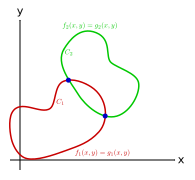
\includegraphics[width = 0.5\textwidth]{intersecting_curves}
}
\end{tabular}


\subsection*{Line Intersections}

\begin{tabular}{cc}
\parbox{0.5\textwidth}{
Consider the {\bf linear} system: 
\[\left\{\begin{array}{c}
A_1x + B_1y = C_1 \\
A_2x + B_2y = C_2
\end{array}\right.\]
where \(A_1\), \(B_1\), \(C_1\), \(A_2\), \(B_2\), and \(C_2\) are all constants. In addition, \(A_1\) and \(B_1\) are not both \(0\), and \(A_2\) and \(B_2\) are not both \(0\).
Each of the equations \(A_1x + B_1y = C_1\) and \(A_2x + B_2y = C_2\) defines a line \(L_1\) and \(L_2\) respectively in the \(x,y\) coordinate system. Each line denotes the set of points that satisfies the line's equation, and points that satisfy both equations are exactly the points that from the intersection between \(L_1\) and \(L_2\). There are 3 possible scenarios:
\begin{itemize}
\item \(L_1\) and \(L_2\) meet at a single point when the system has exactly 1 solution. 
\item \(L_1\) and \(L_2\) are the same line (are coincident) when the system has infinitely many solutions that themselves form a line. 
\item \(L_1\) and \(L_2\) are the parallel, but not coincident, when the system has 0 solutions. 
\end{itemize}
} & \parbox{0.5\textwidth}{
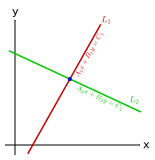
\includegraphics[width = 0.5\textwidth]{line_intersection_scenarios_1_point}
} \\ \parbox{0.5\textwidth}{
\includegraphics[width = 0.5\textwidth]{line_intersection_scenarios_infinite_points}
} & \parbox{0.5\textwidth}{
\includegraphics[width = 0.5\textwidth]{line_intersection_scenarios_0_points}
}
\end{tabular}



\subsection*{Variable elimination via addition}

When solving linear systems that have the form:
\[\left\{\begin{array}{c}
A_1x + B_1y = C_1 \\
A_2x + B_2y = C_2
\end{array}\right.\]
the technique of eliminating variables by ``adding" equations together is often used. Given two equations \(f_1(x,y) = g_1(x,y)\) and \(f_2(x,y) = g_2(x,y)\) the process of ``adding \(k\) times the first equation to the second equation" yields the equation:
\[f_2(x,y) + kf_1(x,y) = g_2(x,y) + kg_1(x,y)\]
Since \(kf_1(x,y) = kg_1(x,y)\), the same quantity has been added to both sides of \(f_2(x,y) = g_2(x,y)\). So the truth of both equations \(f_1(x,y) = g_1(x,y)\) and \(f_2(x,y) = g_2(x,y)\) implies the truth of the the equation \(f_2(x,y) + kf_1(x,y) = g_2(x,y) + kg_1(x,y)\).

Using the addition of equations to solve the linear system is done as follows: If \(A_1 \neq 0\), adding \(-A_2/A_1\) times \(A_1x + B_1y = C_1\) to the equation \(A_2x + B_2y = C_2\) yields the equation:
\[(A_2x + B_2y) - \frac{A_2}{A_1}(A_1x + B_1y) = C_2 - \frac{A_2}{A_1}C_1 \iff (B_2 - \frac{A_2}{A_1}B_1)y = C_2 - \frac{A_2}{A_1}C_1\]
effectively eliminating \(x\) from the equation. For example given the system:
\[\left\{\begin{array}{c}
2x + 3y = 11 \\
6x + 4y = 8 
\end{array}\right.\]
Adding \(-3\) times the first equation to the second equation gives:
\[(6x + 4y) - 3(2x + 3y) = 8 - 3(11) \iff (6 - 6)x + (4 - 9)y = 8 - 33 \iff -5y = -25\]
Variable \(x\) is no longer present in this equation, which instantly gives \(y = 5\). With the value of \(y\) known, any of the initial equations can be used to find \(x\):
\[2x + 3y = 11 \iff 2x + 15 = 11 \iff 2x = -4 \iff x = -2\]




\section*{Linear Programming}

Linear programming is a special case of {\bf constrained optimization}. In constrained optimization, the maximum value of an {\bf objective function} \(f(x,y)\) is sought where the input pair \((x, y)\) is subject to various constraints. An \((x, y)\) pair satisfies all of the constraints is referred to as being {\bf feasible}. 

With {\bf linear programming}, the objective function has the form \(f(x,y) = Ax + By + C\) where \(A\), \(B\), and \(C\) are fixed constants. The constraints are inequalities with the form \(Ex + Fy \geq G\) or \(Ex + Fy \leq G\). Strict inequalities using \(>\) or \(<\) are not allowed. 

The feasible set will always by a {\bf convex polygon}, and the optimal point \((x, y)\) will always be one of the vertices. It should be noted that if two vertices give the same maximum value, then these vertices must be adjacent and all points on the edge between these two vertices are also optimal. In the image below, the same convex polygon is shown as an example feasible set, with different objective functions given. The value of the objective function at each point is determined by the shading, with darker shades corresponding to higher values. On the left the maximum occurs at the single pink colored vertex. On the right, the maximum occurs along the pink colored edge.


\includegraphics[width = \textwidth]{convex_polygon}

The most difficult task in linear programming with two variables is finding the feasible set and all of its vertices. Below are some examples of finding the feasible set with some some objective functions provided at the end.



\subsection*{Example 1}

We will find the feasible set defined by the constraints:
\[\left\{\begin{array}{c} 
3x + y \geq 11 \\
2x - 3y \leq 0 \\
x + 4y \leq 22
\end{array}\right.\]

Each of these constraints will be solved for \(y\) in sequence.

\vspace{5mm}

The first constraint gives:
\[3x + y \geq 11 \iff y \geq -3x + 11\]
The feasible set is bounded from {\bf below} by the line \(L_1\) with equation \(y = -3x + 11\)

\vspace{5mm}

The second constraint gives:
\[2x - 3y \leq 0 \iff -3y \leq -2x \iff y \geq (2/3)x\]
The feasible set is bounded from {\bf below} by the line \(L_2\) with equation \(y = (2/3)x\)

\vspace{5mm}

The third constraint gives:
\[x + 4y \leq 22 \iff 4y \leq -x + 22 \iff y \leq -(1/4)x + 11/2\]
The feasible set is bounded from {\bf above} by the line \(L_3\) with equation \(y = -(1/4)x + 11/2\)

\vspace{5mm}

Lines \(L_1\) and \(L_2\) intersect when \(-3x + 11 = y = (2/3)x\) hence:
\[-3x + 11 = (2/3)x \iff -3x = (2/3)x - 11 \iff -(11/3)x = -11 \iff x = 3\]
\(y = -3x + 11 = 2\) so the intersection between \(L_1\) and \(L_2\) is point \(A(3, 2)\)

\vspace{5mm}

Lines \(L_1\) and \(L_3\) intersect when \(-3x + 11 = y = -(1/4)x + 11/2\) hence:
\[-3x + 11 = -(1/4)x + 11/2 \iff -3x = -(1/4)x - 11/2 \iff -(11/4)x = -11/2 \iff x = 2\]
\(y = -3x + 11 = 5\) so the intersection between \(L_1\) and \(L_3\) is point \(B(2, 5)\)

\vspace{5mm}

Lines \(L_2\) and \(L_3\) intersect when \((2/3)x = y = -(1/4)x + 11/2\) hence:
\[(2/3)x = -(1/4)x + 11/2 \iff (11/12)x = 11/2 \iff x = 6\]
\(y = (2/3)x = 4\) so the intersection between \(L_2\) and \(L_3\) is point \(C(6, 4)\)

\vspace{5mm}

\begin{tabular}{cc}
\parbox{0.5\textwidth}{
A sketch of the feasible set, being a triangle, is shown on the right. The feasible set is the triangle with vertices \(A(3, 2)\), \(B(2, 5)\), and \(C(6, 4)\). The red shaded region is the set of all points that satisfy the first constraint and are above line \(L_1\). The green shaded region is the set of all points that satisfy the second constraint and are above line \(L_2\). The blue shaded region is the set of all points that satisfy the third constraint and are below line \(L_3\). It is important to note that point \(A\) satisfies the third constraint; point \(B\) satisfies the second constraint; and point \(C\) satisfies the first constraint. This ensures that the vertices are actually part of the feasible set. If this were not the case, the triangle would be ``inside out" and the feasible set would be empty.
} & \parbox{0.5\textwidth}{
\includegraphics[width = 0.5\textwidth]{feasible_set_1}
}
\end{tabular}

To find the optimal \((x, y)\), the vertex points are the only candidates \((3, 2)\), \((2, 5)\), and \((6, 4)\).

Now for some example objective functions:
\begin{itemize}
\item If \(f(x, y) = x + y\), then \(f(3, 2) = 5\); \(f(2, 5) = 7\); and \(f(6, 4) = 10\). We can see that \((6, 4)\) is the optimal \((x, y)\) and gives a maximum value of \(10\).
\item If \(f(x, y) = -2x + y\), then \(f(3, 2) = -4\); \(f(2, 5) = 1\); and \(f(6, 4) = -8\). We can see that \((2, 5)\) is the optimal \((x, y)\) and gives a maximum value of \(1\).
\item If \(f(x, y) = -x - 5y\), then \(f(3, 2) = -13\); \(f(2, 5) = -27\); and \(f(6, 4) = -26\). We can see that \((3, 2)\) is the optimal \((x, y)\) and gives a maximum value of \(-13\).
\end{itemize}

\begin{tabular}{cc}
\parbox{0.5\textwidth}{
It is very important to sketch the feasible set. Consider the same constraints but with the inequalities reversed:
\[\left\{\begin{array}{c} 
3x + y \leq 11 \\
2x - 3y \geq 0 \\
x + 4y \geq 22
\end{array}\right.\]
The lines and intersection points remain exactly the same, only feasible points are expected to be below \(L_1\); below \(L_2\); and above \(L_3\). As seen in the image of the right, there is no point that satisfies all three constraints, and the feasible set is empty. Without a sketch of the lines and intersection points, this situation would have been missed.
} & \parbox{0.5\textwidth}{
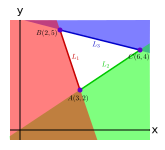
\includegraphics[width = 0.5\textwidth]{feasible_set_1x}
}
\end{tabular}



\subsection*{Example 2}

We will find the feasible set defined by the constraints:
\[\left\{\begin{array}{c} 
(x \geq 0) \wedge (y \geq 0) \\
x + 2y \leq 8 \\
3x + y \leq 9
\end{array}\right.\]

(remember \(\wedge = \text{``AND"}\))

The first constraint forces both \(x\) and \(y\) to be nonnegative, so the feasible region is confined to the positive \(x\), positive \(y\) quadrant. Each of the other constraints will be solved for \(y\) in sequence.

\vspace{5mm}

The second constraint gives:
\[x + 2y \leq 8 \iff 2y \leq -x + 8 \iff y \leq -(1/2)x + 4\]
The feasible set is bounded from {\bf above} by the line \(L_2\) with equation \(y = -(1/2)x + 4\)

\vspace{5mm}

The third constraint gives:
\[3x + y \leq 9 \iff y \leq -3x + 9\]
The feasible set is bounded from {\bf above} by the line \(L_3\) with equation \(y = -3x + 9\)

\vspace{5mm}

The origin is at \(A(0,0)\). 

\vspace{5mm}

Line \(L_2\) intersects the \(y\)-axis when \(x = 0\) which gives \(y = 4\). The \(y\)-intercept is \(B(0,4)\). Line \(L_2\) intersects the \(x\)-axis when \(y = 0\), which occurs when \(-(1/2)x + 4 = 0 \iff -(1/2)x = -4 \iff x = 8\). The \(x\)-intercept is \(C(8,0)\).

\vspace{5mm}

Line \(L_3\) intersects the \(y\)-axis when \(x = 0\) which gives \(y = 9\). The \(y\)-intercept is \(D(0,9)\). Line \(L_3\) intersects the \(x\)-axis when \(y = 0\), which occurs when \(-3x + 9 = 0 \iff -3x = -9 \iff x = 3\). The \(x\)-intercept is \(E(3,0)\).

\vspace{5mm}

Lines \(L_2\) and \(L_3\) intersect when \(-(1/2)x + 4 = y = -3x + 9\) hence:
\[-(1/2)x + 4 = -3x + 9 \iff -(1/2)x = -3x + 5 \iff (5/2)x = 5 \iff x = 2\]
\(y = -(1/2)x + 4 = 3\) so the intersection between \(L_2\) and \(L_3\) is point \(F(2,3)\)

\vspace{5mm}

\begin{tabular}{cc}
\parbox{0.5\textwidth}{
A sketch of the feasible set is shown on the right. The feasible set is above the \(x\)-axis, right of the \(y\)-axis, beneath \(L_2\), and beneath \(L_3\). The vertices of the feasible set consists of \(A(0,0)\), \(B(0,4)\), \(E(3,0)\), and \(F(2,3)\). Points \(C(8,0)\) and \(D(0,9)\) are far outside of the feasible set and are not candidates for the optimal \((x, y)\) point. Ruling out points \(C\) and \(D\) is why a sketch of the feasible set is important. The only candidates for the optimal point are the points \((0,0)\), \((0,4)\), \((3,0)\), and \((2,3)\). 
} & \parbox{0.5\textwidth}{
\includegraphics[width = 0.5\textwidth]{feasible_set_2}
}
\end{tabular}

Now consider the objective function \(f(x, y) = 2x + y\). Evaluating \(f(x, y)\) at each candidate (vertex) point gives:
\begin{itemize}
\item \(f(0, 0) = 0\)
\item \(f(0, 4) = 4\)
\item \(f(3, 0) = 6\)
\item \(f(2, 3) = 7\)
\end{itemize} 
Therefore \((x, y) = (2, 3)\) is the feasible point that maximizes \(f(x, y) = 2x + y\) with a maximum value of \(7\).



\subsection*{Example 3}

We will find the feasible set defined by the constraints:
\[\left\{\begin{array}{c} 
x + 4y \leq 10 \\
4x + y \leq 10 \\
-x + 6y \geq -15 \\
6x - y \geq -15
\end{array}\right.\]

Each of these constraints will be solved for \(y\) in sequence.

\vspace{5mm}

The first constraint gives:
\[x + 4y \leq 10 \iff 4y \leq -x + 10 \iff y \leq -(1/4)x + 5/2\]
The feasible set is bounded from {\bf above} by the line \(L_1\) with equation \(y = -(1/4)x + 5/2\)

\vspace{5mm}

The second constraint gives:
\[4x + y \leq 10 \iff y \leq -4x + 10\]
The feasible set is bounded from {\bf above} by the line \(L_2\) with equation \(y = -4x + 10\)

\vspace{5mm}

The third constraint gives:
\[-x + 6y \geq -15 \iff 6y \geq x - 15 \iff y \geq (1/6)x - 5/2\]
The feasible set is bounded from {\bf below} by the line \(L_3\) with equation \(y = (1/6)x - 5/2\)

\vspace{5mm}

The fourth constraint gives:
\[6x - y \geq -15 \iff -y \geq -6x - 15 \iff y \leq 6x + 15\]
The feasible set is bounded from {\bf above} by the line \(L_4\) with equation \(y = 6x + 15\)

\vspace{5mm}

The intersections between all pairs of lines will be computed:
\begin{itemize}
%%%%%%%%%%%%
\item For \(L_1 \cap L_2\), \(x\) needs to satisfy \(-(1/4)x + 5/2 = -4x + 10\)
\[-(1/4)x + 5/2 = -4x + 10 \iff -(1/4)x = -4x + 15/2 \iff (15/4)x = 15/2 \iff x = 2\]
From \(x = 2\), \(y = -(1/4)x + 5/2 = 2\) so \(L_1 \cap L_2 = A(2, 2)\)
%%%%%%%%%%%%
\item For \(L_1 \cap L_3\), \(x\) needs to satisfy \(-(1/4)x + 5/2 = (1/6)x - 5/2\)
\[-(1/4)x + 5/2 = (1/6)x - 5/2 \iff -(1/4)x = (1/6)x - 5 \iff -(5/12)x = -5 \iff x = 12\]
From \(x = 12\), \(y = -(1/4)x + 5/2 = -1/2\) so \(L_1 \cap L_2 = B(12, -1/2)\)
%%%%%%%%%%%%
\item For \(L_1 \cap L_4\), \(x\) needs to satisfy \(-(1/4)x + 5/2 = 6x + 15\)
\[-(1/4)x + 5/2 = 6x + 15 \iff -(1/4)x = 6x + 25/2 \iff -(25/4)x = 25/2 \iff x = -2\]
From \(x = -2\), \(y = -(1/4)x + 5/2 = 3\) so \(L_1 \cap L_2 = C(-2, 3)\)
%%%%%%%%%%%%
\item For \(L_2 \cap L_3\), \(x\) needs to satisfy \(-4x + 10 = (1/6)x - 5/2\)
\[-4x + 10 = (1/6)x - 5/2 \iff -4x = (1/6)x - 25/2 \iff -(25/6)x = -25/2 \iff x = 3\]
From \(x = 3\), \(y = -4x + 10 = -2\) so \(L_2 \cap L_3 = D(3, -2)\)
%%%%%%%%%%%%
\item For \(L_2 \cap L_4\), \(x\) needs to satisfy \(-4x + 10 = 6x + 15\)
\[-4x + 10 = 6x + 15 \iff -4x = 6x + 5 \iff -10x = 5 \iff x = -1/2\]
From \(x = -1/2\), \(y = -4x + 10 = 12\) so \(L_2 \cap L_4 = E(-1/2, 12)\)
%%%%%%%%%%%%
\item For \(L_3 \cap L_4\), \(x\) needs to satisfy \((1/6)x - 5/2 = 6x + 15\)
\[(1/6)x - 5/2 = 6x + 15 \iff (1/6)x = 6x + 35/2 \iff -(35/6)x = 35/2 \iff x = -3\]
From \(x = -3\), \(y = (1/6)x - 5/2 = -3\) so \(L_3 \cap L_4 = F(-3, -3)\)
\end{itemize}

\vspace{5mm}

\begin{tabular}{cc}
\parbox{0.45\textwidth}{
A sketch of the feasible set is shown on the right. The feasible set is beneath \(L_1\), beneath \(L_2\), above \(L_3\), and beneath \(L_4\). The vertices of the feasible set consists of \(A(2,2)\), \(C(-2,3)\), \(D(3,-2)\), and \(F(-3,-3)\). Points \(B(12,-1/2)\) and \(E(-1/2,12)\) are far outside of the feasible set and are not candidates for the optimal \((x, y)\) point. Ruling out points \(B\) and \(E\) is why a sketch of the feasible set is important. The only candidates for the optimal point are the points \((2,2)\), \((-2,3)\), \((3,-2)\), and \((-3,-3)\). 
} & \parbox{0.55\textwidth}{
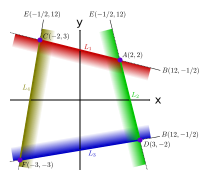
\includegraphics[width = 0.55\textwidth]{feasible_set_3}
}
\end{tabular}

Now consider the objective function \(f(x, y) = 5x + y\). Evaluating \(f(x, y)\) at each candidate (vertex) point gives:
\begin{itemize}
\item \(f(2,2) = 12\)
\item \(f(-2,3) = -7\)
\item \(f(3,-2) = 13\)
\item \(f(-3,-3) = -18\)
\end{itemize} 
Therefore \((x, y) = (3,-2)\) is the feasible point that maximizes \(f(x, y) = 5x + y\) with a maximum value of \(13\).

 


\subsection*{Example 4}

Consider the constraints:
\[\left\{\begin{array}{c}
3 \leq x \leq 5 \\
x - 2y \leq 1 \\
x + y \leq 10
\end{array}\right.\]

The first constraint implies that the feasible set is between the two lines \(x = 3\) and \(x = 5\).

The second constraint \(x - 2y \leq 1\) can be solved to yield:
\[x - 2y \leq 1 \iff -2y \leq -x + 1 \iff y \geq (1/2)x - 1/2\]
The feasible set is therefore bounded from {\bf below} by the line
\[L_2 : y = (1/2)x - 1/2\]

The third constraint \(x + y \leq 10\) can be solved to yield:
\[x + y \leq 10 \iff y \leq -x + 10\]
The feasible set is therefore bounded from {\bf above} by the line
\[L_3 : y = -x + 10\]

Potential vertices of the feasible set include the intersections of \(L_2\) and \(L_3\) with the bounding lines \(x = 3\) and \(x = 5\), and the intersection of \(L_2\) and \(L_3\) with each other. 
\begin{itemize}
\item Line \(L_2\) intersects the line \(x = 3\) when \(x = 3\), so \(y = (1/2)x - 1/2 = 3/2 - 1/2 = 1\), and the intersection point is \(A(3, 1)\). 
\item Line \(L_2\) intersects the line \(x = 5\) when \(x = 5\), so \(y = (1/2)x - 1/2 = 5/2 - 1/2 = 2\), and the intersection point is \(B(5, 2)\). 
\item Line \(L_3\) intersects the line \(x = 3\) when \(x = 3\), so \(y = -x + 10 = 7\), and the intersection point is \(C(3, 7)\). 
\item Line \(L_3\) intersects the line \(x = 5\) when \(x = 5\), so \(y = -x + 10 = 5\), and the intersection point is \(D(5, 5)\). 
\item Lines \(L_2\) and \(L_3\) intersect each other when the values of \(y\) generated by the expressions \(y = (1/2)x - 1/2\) and \(y = -x + 10\) are equal:
\[(1/2)x - 1/2 = -x + 10 \iff (3/2)x = 21/2 \iff x = 7\]
the common value of \(y\) is \(y = 7/2 - 1/2 = 3\), so the intersection point is \(E(7, 3)\).
\end{itemize}

\begin{tabular}{cc}
\parbox{0.5\textwidth}{
A sketch of the feasible set is depicted on the right. The vertices of the feasible set are \(A(3,1)\), \(B(5,2)\), \(C(3,7)\), and \(D(5,5)\). The intersection point \(E(7,3)\) is outside of the feasible set. The candidate points for maximizing the objective function are:
\[(3,1); (5,2); (3,7); (5,5)\]
As an example, given the objective function \(f(x,y) = x + 2y\), evaluating \(f(x,y)\) at each candidate point gives:
\begin{itemize}
\item \(f(3, 1) = 3 + 2 = 5\) 
\item \(f(5, 2) = 5 + 4 = 9\) 
\item \(f(3, 7) = 3 + 14 = 17\) 
\item \(f(5, 5) = 5 + 10 = 15\) 
\end{itemize}
The maximum is \(17\) given by the point \((3, 7)\).
} & \parbox{0.5\textwidth}{
\includegraphics[width = 0.5\textwidth]{feasible_set_4}
}
\end{tabular}
As another example, given the objective function \(f(x,y) = 2x + y\), evaluating \(f(x,y)\) at each candidate point gives:
\begin{itemize}
\item \(f(3, 1) = 6 + 1 = 7\) 
\item \(f(5, 2) = 10 + 2 = 12\) 
\item \(f(3, 7) = 6 + 7 = 13\) 
\item \(f(5, 5) = 10 + 5 = 15\) 
\end{itemize}
The maximum is \(15\) given by the point \((5, 5)\).



\subsection*{Example 5}

Consider the constraints:
\[\left\{\begin{array}{c}
3 \leq x \leq 5 \\
2x - y \leq 5 \\
5x + 2y \leq 29
\end{array}\right.\]

The first constraint implies that the feasible set is between the two lines \(x = 3\) and \(x = 5\).

The second constraint \(2x - y \leq 5\) can be solved to yield:
\[2x - y \leq 5 \iff -y \leq -2x + 5 \iff y \geq 2x - 5\]
The feasible set is therefore bounded from {\bf below} by the line
\[L_2 : y = 2x - 5\]

The third constraint \(5x + 2y \leq 29\) can be solved to yield:
\[5x + 2y \leq 29 \iff 2y \leq -5x + 29 \iff y \leq -(5/2)x + 29/2\]
The feasible set is therefore bounded from {\bf above} by the line
\[L_3 : y = -(5/2)x + 29/2\]

Potential vertices of the feasible set include the intersections of \(L_2\) and \(L_3\) with the bounding lines \(x = 3\) and \(x = 5\), and the intersection of \(L_2\) and \(L_3\) with each other. 
\begin{itemize}
\item Line \(L_2\) intersects the line \(x = 3\) when \(x = 3\), so \(y = 2x - 5 = 6 - 5 = 1\), and the intersection point is \(A(3, 1)\). 
\item Line \(L_2\) intersects the line \(x = 5\) when \(x = 5\), so \(y = 2x - 5 = 10 - 5 = 5\), and the intersection point is \(B(5, 5)\). 
\item Line \(L_3\) intersects the line \(x = 3\) when \(x = 3\), so \(y = -(5/2)x + 29/2 = -15/2 + 29/2 = 14/2 = 7\), and the intersection point is \(C(3, 7)\). 
\item Line \(L_3\) intersects the line \(x = 5\) when \(x = 5\), so \(y = -(5/2)x + 29/2 = -25/2 + 29/2 = 2\), and the intersection point is \(D(5, 2)\). 
\item Lines \(L_2\) and \(L_3\) intersect each other when the values of \(y\) generated by the expressions \(y = 2x - 5\) and \(y = -(5/2)x + 29/2\) are equal:
\[2x - 5 = -(5/2)x + 29/2 \iff (9/2)x = 39/2 \iff x = 39/9 = 13/3\]
the common value of \(y\) is \(y = 26/3 - 5 = 11/3\), so the intersection point is \(E(13/3,11/3)\).
\end{itemize}

\begin{tabular}{cc}
\parbox{0.5\textwidth}{
A sketch of the feasible set is depicted on the right. The vertices of the feasible set are \(A(3, 1)\), \(C(3, 7)\), and \(E(13/3, 11/3)\). The intersection points \(B(5, 5)\) and \(D(5, 2)\) are outside of the feasible set. The candidate points for maximizing the objective function are:
\[(3,1); (3,7); (13/3,11/3)\]
As an example, given the objective function \(f(x,y) = 5x + 3y\), evaluating \(f(x,y)\) at each candidate point gives:
\begin{itemize}
\item \(f(3, 1) = 15 + 3 = 18\) 
\item \(f(3, 7) = 15 + 21 = 36\) 
\item \(f(13/3,11/3) = 65/3 + 33/3 = 98/3 = 32 + 2/3\) 
\end{itemize}
The maximum is \(36\) given by the point \((3, 7)\).
} & \parbox{0.5\textwidth}{
\includegraphics[width = 0.5\textwidth]{feasible_set_5}
}
\end{tabular}




\subsection*{Example 6}

Consider the constraints:
\[\left\{\begin{array}{c}
y \geq 0 \\
2x - y \geq -6 \\
-x + 2y \leq 6 \\
3x + 2y \leq 6
\end{array}\right.\]

The first constraint \(y \geq 0\) implies that the feasible set is above the \(x\)-axis.

The second constraint \(2x - y \geq -6\) can be solved to yield:
\[2x - y \geq -6 \iff -y \geq -2x - 6 \iff y \leq 2x + 6\]
The feasible set is therefore bounded from {\bf above} by the line
\[L_2 : y = 2x + 6\]

The third constraint \(-x + 2y \leq 6\) can be solved to yield:
\[-x + 2y \leq 6 \iff 2y \leq x + 6 \iff y \leq (1/2)x + 3\]
The feasible set is therefore bounded from {\bf above} by the line
\[L_3 : y = (1/2)x + 3\]

The fourth constraint \(3x + 2y \leq 6\) can be solved to yield:
\[3x + 2y \leq 6 \iff 2y \leq -3x + 6 \iff y \leq -(3/2)x + 3\]
The feasible set is therefore bounded from {\bf above} by the line
\[L_4 : y = -(3/2)x + 3\]

Potential vertices of the feasible set include the intersections of \(L_2\), \(L_3\), and \(L_4\) with the \(x\)-axis, and the intersections of these lines with each other.
\begin{itemize}
%%%%%%%%%%%%%%
\item Line \(L_2\) intersects the \(x\)-axis when \(y = 0\), so finding the \(x\)-coordinate requires solving the equation \(2x + 6 = 0\)
\[2x + 6 = 0 \iff 2x = -6 \iff x = -3\] 
The intersection point is \(A(-3, 0)\).
%%%%%%%%%%%%%%
\item Line \(L_3\) intersects the \(x\)-axis when \(y = 0\), so finding the \(x\)-coordinate requires solving the equation \((1/2)x + 3 = 0\)
\[(1/2)x + 3 = 0 \iff (1/2)x = -3 \iff x = -6\] 
The intersection point is \(B(-6, 0)\). 
%%%%%%%%%%%%%%
\item Line \(L_4\) intersects the \(x\)-axis when \(y = 0\), so finding the \(x\)-coordinate requires solving the equation \(-(3/2)x + 3 = 0\)
\[-(3/2)x + 3 = 0 \iff -(3/2)x = -3 \iff x = 2\]
The intersection point is \(C(2, 0)\).   
%%%%%%%%%%%%%%
\item Lines \(L_2\) and \(L_3\) intersect each other when the values of \(y\) generated by the expressions \(y = 2x + 6\) and \(y = (1/2)x + 3\) are equal:
\[2x + 6 = (1/2)x + 3 \iff (3/2)x = -3 \iff x = -2\]      
the common value of \(y\) is \(y = -4 + 6 = 2\), so the intersection point is \(D(-2, 2)\). 
%%%%%%%%%%%%%%
\item Lines \(L_2\) and \(L_4\) intersect each other when the values of \(y\) generated by the expressions \(y = 2x + 6\) and \(y = -(3/2)x + 3\) are equal:
\[2x + 6 = -(3/2)x + 3 \iff (7/2)x = -3 \iff x = -6/7\]
the common value of \(y\) is \(y = -12/7 + 6 = 30/7\), so the intersection point is \(E(-6/7, 30/7)\).
%%%%%%%%%%%%%%
\item Lines \(L_3\) and \(L_4\) intersect each other when the values of \(y\) generated by the expressions \(y = (1/2)x + 3\) and \(y = -(3/2)x + 3\) are equal:  
\[(1/2)x + 3 = -(3/2)x + 3 \iff 2x = 0 \iff x = 0\]
the common value of \(y\) is \(y = 3\), so the intersection point is \(F(0, 3)\).
\end{itemize}

\begin{tabular}{cc}
\parbox{0.4\textwidth}{
A sketch of the feasible set is depicted on the right. The vertices of the feasible set are \(A(-3,0)\), \(C(2,0)\), \(D(-2,2)\), and \(F(0,3)\). The intersection points \(B(-6,0)\) and \(E(-6/7,30/7)\) are outside of the feasible set. The candidate points for maximizing the objective function are:  
\[(-3,0); (2,0); (-2,2); (0,3)\]
As an example, given the objective function \(f(x,y) = -x + y\), evaluating \(f(x,y)\) at each candidate point gives:
\begin{itemize}
\item \(f(-3,0) = 3\)
\item \(f(2,0) = -2\)
\item \(f(-2,2) = 4\)
\item \(f(0,3) = 3\)
\end{itemize}
The maximum is \(4\) given by the point \((-2, 2)\).
} & \parbox{0.6\textwidth}{
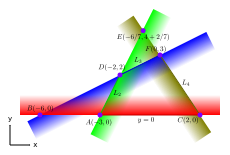
\includegraphics[width = 0.6\textwidth]{feasible_set_6}
}
\end{tabular}




\section*{An Application of Linear Programming}

\subsection*{Data}

\begin{itemize}
\item Each unit of toy 1 sells for \(\textbf{price}_1 = \$15.00\), and costs \(\textbf{labor}_1 = \$4.00\) in labor, and requires \(\textbf{plas}_1 = 2.0\text{kg}\) of plastic and \(\textbf{metal}_1 = 1.0\text{kg}\) of metal. 
\item Each unit of toy 2 sells for \(\textbf{price}_2 = \$25.00\), and costs \(\textbf{labor}_2 = \$4.00\) in labor, and requires \(\textbf{plas}_2 = 4.0\text{kg}\) of plastic and \(\textbf{metal}_2 = 0.5\text{kg}\) of metal. 
\item The cost of plastic is \(\textbf{cost\_plas\_kg} = \$1.00/\text{kg}\), and the cost of metal is \(\textbf{cost\_metal\_kg} = \$4.00/\text{kg}\). 
\item The total budget is \(\textbf{budget} = \$20,\!000.00\). 
\item The total supply of plastic is \(\textbf{plas\_limit} = 7,\!000\text{kg}\). 
\item The total supply of metal is \(\textbf{metal\_limit} = 1,\!750\text{kg}\). 
\end{itemize}

The number of units of toy 1, denoted by \(x\), and the number of units of toy 2, denoted by \(y\), that maximizes the profits \(z\) are sought.


\subsection*{Calculations}

The cost of the plastic in toy 1 and toy 2 is respectively:
\begin{align*}
& \textbf{plas\_cost}_1 = \textbf{plas}_1 \cdot \textbf{cost\_plas\_kg} = \$2.00 \\
& \textbf{plas\_cost}_2 = \textbf{plas}_2 \cdot \textbf{cost\_plas\_kg} = \$4.00
\end{align*}

The cost of the metal in toy 1 and toy 2 is respectively:
\begin{align*}
& \textbf{metal\_cost}_1 = \textbf{metal}_1 \cdot \textbf{cost\_metal\_kg} = \$4.00 \\
& \textbf{metal\_cost}_2 = \textbf{metal}_2 \cdot \textbf{cost\_metal\_kg} = \$2.00
\end{align*}

The total cost of producing a unit of toy 1 is:
\[\textbf{cost}_1 = \textbf{labor}_1 + \textbf{plas\_cost}_1 + \textbf{metal\_cost}_1 = \$10.00\]
The total cost of producing a unit of toy 2 is:
\[\textbf{cost}_2 = \textbf{labor}_2 + \textbf{plas\_cost}_2 + \textbf{metal\_cost}_2 = \$10.00\]

\vspace{5mm}

The total profit per unit of toy 1 sold is:
\[\textbf{profit}_1 = \textbf{price}_1 - \textbf{cost}_1 = \$5.00\]
The total profit per unit of toy 2 sold is:
\[\textbf{profit}_2 = \textbf{price}_2 - \textbf{cost}_2 = \$15.00\]

\vspace{5mm}

It is already clear that \(x \geq 0\) and \(y \geq 0\). 

\vspace{5mm}

The budget sets the limit:
\[\textbf{cost}_1 x + \textbf{cost}_2 y \leq \textbf{budget}\] 

\vspace{5mm}

The plastic supply sets the limit:
\[\textbf{plas}_1 x + \textbf{plas}_2 y \leq \textbf{plas\_limit}\]

\vspace{5mm}

The metal supply sets the limit:
\[\textbf{metal}_1 x + \textbf{metal}_2 y \leq \textbf{metal\_limit}\]

\vspace{5mm}

The constraints are therefore:
\[\left\{\begin{array}{c}
x, y \geq 0 \\
\textbf{cost}_1 x + \textbf{cost}_2 y \leq \textbf{budget} \\
\textbf{plas}_1 x + \textbf{plas}_2 y \leq \textbf{plas\_limit} \\
\textbf{metal}_1 x + \textbf{metal}_2 y \leq \textbf{metal\_limit}
\end{array}\right.\] 

end the objective function is:
\[z = \textbf{profit}_1x + \textbf{profit}_2y\]

\vspace{5mm}

The constraints \(x, y \geq 0\) limits the feasible set to the positive \(x\), positive \(y\) quadrant. 

\vspace{5mm}

Solving the budget constraint for \(y\) gives:
\begin{align*}
& \textbf{cost}_1 x + \textbf{cost}_2 y \leq \textbf{budget} \\ 
\iff & \textbf{cost}_2 y \leq \textbf{budget} - \textbf{cost}_1 x \\
\iff & y \leq \textbf{budget}/\textbf{cost}_2 - (\textbf{cost}_1/\textbf{cost}_2)x
\end{align*}
so the feasible set is bounded from above by the line 
\[L_\text{budget} : \quad y = \textbf{budget}/\textbf{cost}_2 - (\textbf{cost}_1/\textbf{cost}_2)x\]
This line is: \(y = m_\text{budget}x + c_\text{budget}\) where \(m_\text{budget} =  -(\textbf{cost}_1/\textbf{cost}_2) = -1\) and \(c_\text{budget} = \textbf{budget}/\textbf{cost}_2 = 2000\)

\vspace{5mm}

Solving the plastic constraint for \(y\) gives:
\begin{align*}
& \textbf{plas}_1 x + \textbf{plas}_2 y \leq \textbf{plas\_limit} \\ 
\iff & \textbf{plas}_2 y \leq \textbf{plas\_limit} - \textbf{plas}_1 x \\
\iff & y \leq \textbf{plas\_limit}/\textbf{plas}_2 - (\textbf{plas}_1/\textbf{plas}_2)x
\end{align*}
so the feasible set is bounded from above by the line 
\[L_\text{plas} : \quad y = \textbf{plas\_limit}/\textbf{plas}_2 - (\textbf{plas}_1/\textbf{plas}_2)x\]
This line is: \(y = m_\text{plas}x + c_\text{plas}\) where \(m_\text{plas} =  -(\textbf{plas}_1/\textbf{plas}_2) = -0.5\) and \(c_\text{plas} = \textbf{plas\_limit}/\textbf{plas}_2 = 1750\)

\vspace{5mm}

Solving the metal constraint for \(y\) gives:
\begin{align*}
& \textbf{metal}_1 x + \textbf{metal}_2 y \leq \textbf{metal\_limit} \\ 
\iff & \textbf{metal}_2 y \leq \textbf{metal\_limit} - \textbf{metal}_1 x \\
\iff & y \leq \textbf{metal\_limit}/\textbf{metal}_2 - (\textbf{metal}_1/\textbf{metal}_2)x
\end{align*}
so the feasible set is bounded from above by the line 
\[L_\text{metal} : \quad y = \textbf{metal\_limit}/\textbf{metal}_2 - (\textbf{metal}_1/\textbf{metal}_2)x\]
This line is: \(y = m_\text{metal}x + c_\text{metal}\) where \(m_\text{metal} =  -(\textbf{metal}_1/\textbf{metal}_2) = -2\) and \(c_\text{metal} = \textbf{metal\_limit}/\textbf{metal}_2 = 3500\)

\vspace{5mm}

Since the \(x\) and \(y\) axes bound the feasible set, the \(x\) and \(y\) intercept points for each line are important. Given an arbitrary line \(y = mx + c\), the \(y\)-intercept occurs at \((0, c)\), and the \(x\)-intercept occurs when \(y = 0\):
\[y = 0 \iff mx + c = 0 \iff mx = -c \iff x = -c/m\]
Hence the \(x\)-intercept occurs at \((-c/m, 0)\). 

For line \(L_\text{budget}\), the \(x\) and \(y\) intercept points are respectively: 
\begin{align*}
& A_\text{budget}(-c_\text{budget}/m_\text{budget}, 0) = A_\text{budget}(2000, 0)\\
& B_\text{budget}(0, c_\text{budget}) = B_\text{budget}(0, 2000)
\end{align*}

For line \(L_\text{plas}\), the \(x\) and \(y\) intercept points are respectively: 
\begin{align*}
& A_\text{plas}(-c_\text{plas}/m_\text{plas}, 0) = A_\text{plas}(3500, 0)\\
& B_\text{plas}(0, c_\text{plas}) = B_\text{plas}(0, 1750)
\end{align*}

For line \(L_\text{metal}\), the \(x\) and \(y\) intercept points are respectively: 
\begin{align*}
& A_\text{metal}(-c_\text{metal}/m_\text{metal}, 0) = A_\text{metal}(1750, 0)\\
& B_\text{metal}(0, c_\text{metal}) = B_\text{metal}(0, 3500)
\end{align*}

\vspace{5mm}

Now to find the intercept points between each pair of lines. Given an arbitrary pair of lines \(y = m_1x + c_1\) and \(y = m_2x + c_2\), the lines intersect when \(m_1x + c_1 = y = m_2x + c_2\):
\[m_1x + c_1 = m_2x + c_2 \iff (m_1 - m_2)x = c_2 - c_1 \iff x = \frac{c_2 - c_1}{m_1 - m_2}\]
so:
\[y = m_1x + c_1 = \frac{m_1c_2 - m_1c_1}{m_1 - m_2} + \frac{m_1c_1 - m_2c_1}{m_1 - m_2} = \frac{m_1c_2 - m_2c_1}{m_1 - m_2}\]
The intersection point is:
\[\left(\frac{c_2 - c_1}{m_1 - m_2}, \frac{m_1c_2 - m_2c_1}{m_1 - m_2}\right)\] 

Using this formula, the intersection between \(L_\text{budget}\) and \(L_\text{plas}\) is \(C(500, 1500)\); the intersection between \(L_\text{budget}\) and \(L_\text{metal}\) is \(D(1500, 500)\); the intersection between \(L_\text{plas}\) and \(L_\text{metal}\) is \(E(1166.67, 1166.67)\)

\begin{tabular}{cc}
\parbox{0.5\textwidth}{
The feasible set is sketched on the right. The vertices of the feasible set are the points \((0, 0)\); \(B_\text{plas}(0, 1750)\); \(A_\text{metal}(1750, 0)\); \(C(500, 1500)\); and \(D(1500, 500)\). Evaluating the profit \(z = \textbf{profit}_1x + \textbf{profit}_2y\) at each vertex gives:
\begin{itemize}
\item \((x, y) = (0, 0) \implies z = \$0\)
\item \((x, y) = (0, 1750) \implies z = \$26250\)
\item \((x, y) = (1750, 0) \implies z = \$8750\)
\item \((x, y) = (500, 1500) \implies z = \$25000\)
\item \((x, y) = (1500, 500) \implies z = \$15000\)
\end{itemize}
The profit is maximized when \(x = 0\) units of toy 1 are manufactured and \(y = 1750\) units of toy 2 are manufactured. The maximum profit is \(z = \$26250\). 
} & \parbox{0.5\textwidth}{
\includegraphics[width = 0.5\textwidth]{feasible_set_application}
}
\end{tabular}



\end{document}













